\documentclass{elsinta}
\usepackage{url}

% --- Memasukkan Data Dokumen Menggunakan Perintah Baru ---
\projectcode{EL2}
\documentname{\LiteraturesStandardsTitle}
\documenttitle{Teknik Elektro - Sistem Informasi Tugas Akhir}
\capstonetitle{Monitoring On Induction Motor In Real-Time: Vibration and Temperature}
\shortname{MONTREAL-VT} 
\documentnumber{TA2526.02.003}
\revisionnumber{02}
\publicationdate{2 September 2026}
\revdatefooter{6/7/2026}
% --- Memasukkan Data Halaman Pengesahan (Halaman 2) ---
\currentpage{2} % Halaman yang sedang dicetak

% Data Tim
\ketuatimnama{Mahasiswa 1}
\ketuatimnim{12345678}

\anggotanamaI{Mahasiswa 2}
\anggotanimI{12345678}

\anggotanamaII{Mahasiswa 3}
\anggotanimII{12345678}


% Data Dosen
\pembimbingInama{Dosen 1}
\pembimbingInip{12345678 123456 1 123}

\pembimbingIInama{Dosen 2}
\pembimbingIInip{12345678 123456 1 123}


% Tanggal Pengesahan
\approvaldate{22 September 2025}

\begin{document}

% Panggil perintah untuk membuat halaman sampul
\coverpage
% Pindah ke Halaman Baru
\newpage

% Membuat Halaman Pengesahan (Halaman 2)
% \approvalpage

% Lanjut ke halaman proposal
% \newpage

% ======================================
% Bagian Konten Proposal Dimulai di Sini
% ======================================

% Mengatur ulang nomor halaman dan gaya halaman
\clearpage
\pagenumbering{arabic}
\setcounter{page}{1} 
\pagestyle{myfooter} % Ganti dari 'plain' ke 'myfooter'

% Atur margin standar (Opsional, jika Anda ingin margin isi berbeda dari sampul)
% \newgeometry{left=4cm, right=3cm, top=3cm, bottom=3cm} 
% Catatan: Perintah \newgeometry memerlukan paket 'geometry' yang sudah ada di cls.

\tableofcontents
\newpage
\section*{\docsumary}
Dokumen ini menyajikan kajian pustaka, analisis kesenjangan serta standar dan regulasi yang menjadi landasan dalam pengembangan proyek \textbf{Monitoring on Induction Motor in Real-Time: Vibration and Temperature (MONTREAL-VT)}.

Kajian diawali dengan identifikasi produk
komersial, paten, dan penelitian terdahulu 
yang relevan sebagai evaluasi perkembangan 
teknologi pemantauan kondisi mesin, khususnya 
pada aspek pengukuran getaran, suhu, 
komunikasi IoT, dan diagnostik kerusakan.

Hasil studi literatur yang dilakukan menunjukkan bahwa
terdapat keterbatasan pada solusi yang ada,
hal ini meliputi; tinggia biaya implementasi,
rumitnya proses diagnostik sehingga membutuhkan
jasa ahli, serta ketiadaan
sistem alarm dan proteksi otomatis pada sistem.
Hal ini menjadi landasan agar pengembangan MONTREAL-VT
akan berkontribusi untuk mengisi kekurangan pada sistem yang sudah ada.

Beberapa dokumen yang menjadi standar internasional seperti
ISO 20816, ISO 13373, dan IEC 60034 dirujuk agar fungsi
alat yang dirancang sesuai dengan standar yang berlaku. 
Pertimbangan pada analisis getaran meliputi bagian yang dipantau;
rotating atau non-rotating, metode analisis; time-domain, frequency-domain,
dan/atau envelope analysis. Serta menunjukkan batas suhu maksimum
dan batas kenaikan suhu maksimum pada winding.

\newpage

\section{\ProjectBenchmarkTitle}
% Bagian ini menyajikan tinjauan komprehensif terhadap solusi, proyek, penelitian, atau paten terdahulu yang relevan dengan topik proyek Sistem Monitoring Getaran dan Suhu Motor Induksi. Tujuannya adalah untuk memahami kondisi teknologi terkini, mengidentifikasi celah (gap), dan menegaskan improvisasi dari proyek yang diusulkan.

\subsection{\PrevProjectsTitle}
% Subbab ini membahas sistem atau proyek yang telah diimplementasikan, baik secara komersial maupun sebagai prototipe, yang memiliki fungsi serupa.

    % \begin{figure}[b!]
    %     \centering
    %     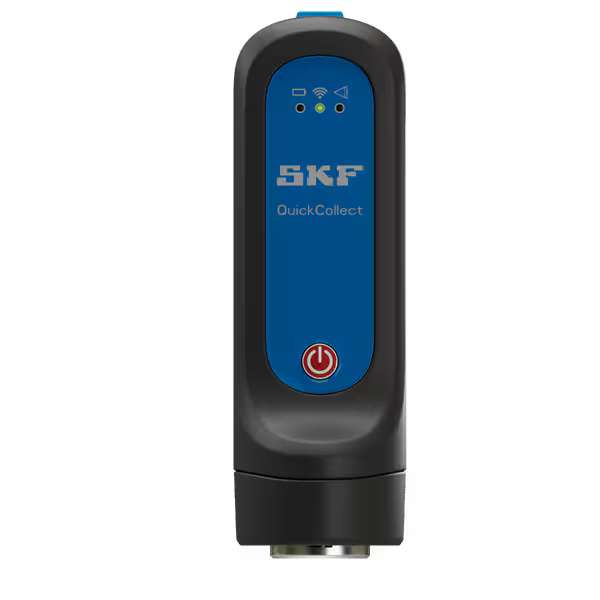
\includegraphics[width=0.5\textwidth]{image/doc/cmdt391.png}
    %     \caption{Sensor QuickCollect CMDT 391}
    %     \label{fig:fishbone}
    % \end{figure}

\subsubsection*{Identifikasi Solusi Terdahulu:}
\begin{enumerate}
    \item \textbf{SKF QuickCollect CMDT 391 (Komersial):}
    \begin{enumerate}
        \item \textbf{Fitur:} Sensor getaran, kondisi bearing, dan suhu terpadu yang mampu diintegrasikan dengan aplikasi pemantauan cloud terkoneksi android dan iOS \cite{SKFGroup2021}, wujud produk ditampilkan pada gambar EL2.1.
        \item \textbf{Kelebihan:} Maksimum percepatan ($50g$), rentang frekuensi internal sensor ($\leq f \leq 10000Hz$), \textit{sample rate} ($256\leq sr \leq 32768$) sampel \cite{SKFGroup2025}, aplikasi mudah dioperasikan pengguna.
        \item \textbf{Kekurangan:} Harga sangat mahal yang berkisar $Rp26.000.000,00$ hingga $Rp50.000.000,00$, solusi berlebihan untuk sistem skala Usaha Mikro, Kecil, dan Menengah (UMKM).
        \item \textbf{Celah produk:} Mengembangkan solusi pemantauan motor induksi minim biaya yang dilengkapi aplikasi pemantauan yang mampu dioperasikan jarak jauh.
    \end{enumerate}
    \item \textbf{Siemens SIDRIVE IQ (Komersial):}
    \begin{enumerate}
        \item \textbf{Fitur:} Jasa IoT industri dalam pemantauan kondisi, \textit{Preventive Maintenance} (PM), analisis kegagalan reaktif \cite{SiemensAG2023}.
        \item \textbf{Kelebihan:} Sistem analitik berbasis IoT dengan dukungan kendali jarak jauh, \textit{Motor Damage Detection System}, Pemodelan numerik berbasis \textit{Internet of Things} (IoT) cloud\cite{SiemensAG2023}.
        \item \textbf{Kekurangan:} Sistem SIDRIVE IQ dilakukan melalui platform cloud Siemens, biaya implementasi tinggi sehingga tidak cocok untuk industri tingkat UMKM, ekosistem yang bersifat \textit{vendor lock-in}, algoritma analistik yang bersifat eksklusif.
        \item \textbf{Celah produk:} Merancang sistem pemantauan kondisi motor induksi berbasis sensor getaran dan sensor suhu yang berbiaya rendah sehingga mampu diakses bisnis skala UMKM. Mengembangkan model yang mampu dilatih menggunakan data motor induksi sehingga mampu mendeteksi kerusakan dan melakukan klasifikasi kerusakan pada motor induksi.
    \end{enumerate}
\end{enumerate}
 
\subsection{\RelResearchPatentsTitle}
% Subbab ini mengulas penelitian ilmiah dan paten yang telah dipublikasikan terkait teknologi atau metodologi yang akan digunakan.
\begin{enumerate}
    \item \textbf{Paten:} Metode Pemantauan Getaran Rotating Equipment secara Real-Time dengan Pemrosesan FFT menggunakan Mikrokontroler (distribusi approval)\cite{Silaban2026}.
    \begin{enumerate}
        \item \textbf{Studi:} Paten ini mengusulkan metode pemantauan getaran dan mikrokontroler ESP32 yang mengimplementasikan algoritma \textit{Fast-Fourier Transform} (FFT). Data getaran yang diperoleh sensor diproses secara \textit{real-time} pada mikrokontroler sehingga menghasilkan representasi domain waktu dan domain frekuensi. Data ini memungkinkan identfikasi karakteristik getaran.
        \item \textbf{Relevansi dengan  MONTREAL-VT:} Paten ini menjadi landasan dalam implementasi pengolahan data yang diperoleh sensor getaran menjadi informasi kondisi motor induksi satu-fasa. Proses FFT merupakan proses konversi data getaran domain waktu menjadi domain frekuensi.
        \item \textbf{Kontribusi  MONTREAL-VT:} Mengimplementasikan pemrosesan sinyal getaran dan mengembangkan algoritma konversi domain waktu yang merepresentasikan getaran ke domain frekuensi guna mendapatkan informasi kondisi motor induksi satu-fasa. MONTREAL-VT juga dilengkapi dengan fitur klasifikasi keparahan getaran dengan mengacu pada standar \textit{International Organization for Standardization} (ISO).
        % visualisasi data pada laman web berbasis cloud, serta mengembangkan algoritma diagnostik berbasis parameter getaran dan suhu.
    \end{enumerate}
    \item \textbf{Riset:} \textit{Health Monitoring of Induction Motor through Vibration Analysis} \cite{Sonowal2019}
    \begin{enumerate}
        \item \textbf{Studi:} Penelitian ini menerapkan \textit{Vibration Analysis Technique} (VAT) sebagai pendekatan Non-Destructive Testing (NDT) untuk memantau kondisi motor induksi tiga-fasa. Sistem dikembangkan menggunakan mikrokontroler dan sensor akselerometer untuk memperoleh sinyal percepatan getaran.
        \item \textbf{Relevansi dengan  MONTREAL-VT:} Metodologi VAT menjadi dasar dalam proses akuisisi data getaran dari motor induksi. MONTREAL-VT mengadopsi sensor getaran sebagai media pengumpulan data.
        \item \textbf{Kontribusi  MONTREAL-VT:} MONTREAL-VT memperluas pendekatan riset\cite{Sonowal2019} dengan parameter tambahan seperti rpm, suhu, dan arus sehingga proses diagnosis tidak hanya mengandalkan data getaran motor. MONTREAL-VT dibekali sistem peunggahan data berbasis cloud sehingga pengguna dapat mengakses data hasil akuisisi dan diagnosa kondisi motor.
    \end{enumerate}
    \item \textbf{Riset:} \textit{Monitoring of Single-Phase Induction Motor through IoT Using ESP32 Module} \cite{Shukla2022}
    \begin{enumerate}
        \item \textbf{Studi:} Shukla et al. mengembangkan sistem pemantauan pada motor induksi multi-parameter dengan memanfaatkan sensor akselerometer, sensor arus, dan sensor suhu.
        \item \textbf{Relevansi dengan MONTREAL-VT:} Penelitian ini mengembangkan sistem pemantauan kondisi motor induksi satu-fasa multi-parameter menggunakan mikrokontroler yang terintegrasi IoT untuk memperoleh dan bertukar informasi, serta mampu dioperasikan dari jarak jauh.
        \item \textbf{Kontribusi MONTREAL-VT:} MONTREAL-VT menngembangkan proses pengolahan data dan konversi ke data domain frekuensi secara \textit{real-time}. MONTREAL-VT dilengkapi dengan fitur notifikasi kondisi motor yang didasarkan pada kombinasi tren data arus, rpm, dan suhu sehingga sistem tidak hanya menampilkan hasil pengukuran sensor tetapi juga memberikan informasi mengenai kondisi motor.
    \end{enumerate}
    \item \textbf{Riset:} \textit{IoT-Based Real-Time Vibration and Temperature Monitoring System for Industrial Machinery Using ESP32 and MQTT}\cite{Shiddiqi2026}
    \begin{enumerate}
        \item \textbf{Studi:} Kontribusi utama dari riset ini merupakan implementasi klasifikasi keparahan getaran dengan mengacu pada standar ISO, integrasi akuisisi multi-sensor dengan pemrosesan RMS dan FFT secara \textit{real-time} tanpa menitikberatkan pada algoritma \textit{machine learning} (ML).
        \item \textbf{Relevansi dengan MONTREAL-VT:} Penelitian ini menjadi referensi dalam implementasi pemrosesan data domain waktu menjadi domain frekuensi secara \textit{real-time} dengan mengacu pada standar ISO 13373 dan ISO 20816, implementasi protokol komunikasi IoT, serta model klasifikasi keparahan getaran dengan mengacu pada ISO 20816 sebagai dasar evaluasi tingkat keparahan getaran pada sistem pemantauan kondisi mesin.
        \item \textbf{Kontribusi MONTREAL-VT:} MONTREAL-VT menerapkan pemrosesan sinyal getaran seperti pemfilteran, penguatan, dan konversi data getaran domain waktu ke domain frekuensi yang diintegrasikan model klasifikasi keparahan getaran ISO 20816-1:2016.
    \end{enumerate}
    \item \textbf{Riset:} Rancang Bangun Sistem Deteksi Menggunakan Getaran, Suhu, Arus, dan rpm Motor Listrik\cite{Yusro2025}
    \begin{enumerate}
        \item \textbf{Studi:} Silaban et al. pada risetnya mengembangkan sistem dengan nama \textit{MachinaSense Predictive Enginer Guardian} yang berfungsi sebagai sistem pemantauan kondisi mesin yang dilakukan secara kontinyu. Sistem ini mengintegrasikan beberapa sensor yang meliputi sensor suhu, sensor rpm \textit{Rotary Encoder}, dan sensor getaran yang dikontrol menggunakan mikrokontroler (ESP32).
        \item \textbf{Relevansi dengan MONTREAL-VT:} Penelitian ini menjadi referensi pengembangan sistem multisensor yang memadukan beberapa parameter operasional mesin untuk meningkatkan akurasi diagnostik.
        \item \textbf{Kontribusi MONTREAL-VT:} MONTREAL-VT menyajikan algoritma analisis spektrum getaran FFT yang sesuai dengan standar teknis internasional seperti ISO 20816 dan ISO 13373.
    \end{enumerate}
    \item \textbf{Riset:} Desain Sistem Monitoring Gangguan Motor Induksi Berdasarkan Nilai Suhu, Getaran, dan Konsumsi Arus\cite{Silaban2026}
    \begin{enumerate}
        \item \textbf{Studi:} Paper ini menyajikan desain sistem pemantauan berbasis IoT yang terhubung melalui \textit{Local Area Network }(LAN). Sistem ini terdiri atas ESP8266 menggunakan arsitektur komunikasi \textit{master-slave}. Sistem mengintegrasikan sensor DS18B20, MPU6050, lalu sensor arus SCT013-30A. Proses penyimpnanan data memanfaatkan MySQL dan ditampilkan pada web server lokal. Riset ini menjadikan ISO 10813 sebagai landasan klasifikasi status motor.
        \item \textbf{Relevansi dengan MONTREAL-VT:} Penelitian ini menjadi referensi dalam integrasi multisensor untuk pemantauan kondisi motor induksi serta implementasi database cloud sebagai media penyimpnanan, visualisasi data, dan media akses data secara \textit{real-time} dan jarak jauh.
        \item \textbf{Kontribusi MONTREAL-VT:} MONTREAL-VT mengimplementasikan protokol MQTT dengan penyimpanan data pada platform cloud, menerapkan FFT, serta mengimplementasikan klasifikasi kondisi motor sehingga sistem mampu memberikan informasi diagnostik mengenai kondisi motor.
    \end{enumerate}
\end{enumerate}

\section{\GapAnalysisTitle}
% Berdasarkan tolok ukur proyek pada bagian sebelumnya, subbab ini akan secara spesifik mengidentifikasi kesenjangan atau celah yang ada pada solusi/penelitian terdahulu. Analisis ini sangat penting untuk memvalidasi improvisasi yang dihasilkan proyek yang diusulkan, dengan menunjukkan bagaimana proyek ini akan mengisi celah-celah tersebut dan memberikan kontribusi yang berarti.

\subsection{\LimitationsTitle}
% Solusi-solusi  yang ada saat ini, baik produk komersial maupun prototipe hasil penelitian sebelumnya, memiliki beberapa keterbatasan kunci yang belum sepenuhnya teratasi. Contoh Keterbatasan:
\begin{enumerate}
    \item \textbf{Biaya Implementasi yang relatif tinggi bagi UMKM dan laboratorium pendidikan:} Solusi yang ada saat ini seperti SKF CMDT391\cite{SKFGroup2021} dan layanan Siemens SIDRIVE IQ\cite{SiemensAG2023} umumnya dirancang untuk aplikasi industri berskala besar dengan biaya investasi, lisensi, dan pemeliharaan yang relatif tinggi. Solusi tersebut berlebihan untuk industri kecil dan menengah, laboratorium pendidikan, maupun lingkungan penelitian.
    \item \textbf{Sistem kurang memiliki klasifikasi kerusakan yang detil:} Sistem pemantauan berbasis IoT yang hanya berfungsi sebagai alat akuisisi dan visualisasi data tanpa dibekali algoritma yang dapat mengidentifikasi jenis kerusakan secara langsung\cite{Sonowal2019}, beberapa sistem dibekali dengan identifikasi status motor yang kurang detil (contoh: waspada, aman)\cite{Yusro2025, Silaban2026}. Akibatnya, pengguna masih harus melakukan interpretasi data secara manual untuk mengidentifikasi bagian motor yang mengalami kerusakan. 
    \item \textbf{Proses penyimpanan dan pemrosesan masih dilakukan secara lokal:} Sebagian sistem masih menyimpan dan mengolah data secara lokal\cite{Silaban2026, Sonowal2019, Yusro2025}, sehingga proses penyimpanan dan pengolahan data sinyal getaran terlalu membebani mikrokontroler.
    \item \textbf{Sistem yang tidak dibekali sistem proteksi:} Sebagian sistem pemantauan kondisi motor hanya menyajikan data, dan informasi motor\cite{Sonowal2019, Silaban2026, Yusro2025}. Sistem pemantauan kondis yang baik memiliki komponen proteksi seperti \textit{Molded Case Circuit Breake}r (MCCB) atau \textit{Thermal Overload Relay} (TOR) sehingga mampu memutus sumber arus dari motor dalam kondisi waspada.
\end{enumerate}

\subsection{\ProjectContribsTitle}
% Sub-bab ini secara eksplisit mengidentifikasi dan mendokumentasikan \textbf{kontribusi} yang dihasilkan oleh Proyek Capstone ini. Contoh celah yang diisi oleh project:
\begin{enumerate}
    \item \textbf{Sistem pemantauan kondisi Motor induksi biaya rendah berbasis sensor getaran dan sensor suhu:} Proyek MONTREAL-VT mengembangkan sistem pemantauan kondisi motor induksi berbasis getaran dan suhu dengan memanfaatkan ESP32 dan integrasi sensor akselerometer, sensor suhu, sensor arus, dan sensor tegangan untuk memperoleh informasi kondisi motor.
    \item \textbf{Sistem klasifikasi kerusakan detil hingga prediksi kerusakan bagian motor:} MONTREAL-VT dibekali algoritma yang mampu menyajikan data, dan prediksi kerusakan hingga ke bagian motor dan dilengkapi dengan saran tindakan untuk mengatasi kerusakan. Algoritma prediksi kerusakan ini berlandaskan seri ISO 20813 dan 13373, dan IEC 60034 untuk suhu.
    \item \textbf{Sistem penyimpanan dan pemrosesan data menggunakan cloud-IoT:} MONTREAL-VT menerapkan sistem penyimpanan dan pemrosesan data berbasis cloud sehingga tidak membebani mikrokontroler terlalu berat. Data hasil visualisasi, diagnosis, dan saran tindakan dapat diakses secara daring oleh pengguna.
    \item \textbf{Sistem yang dilengkapi proteksi:} MONTREAL-VT dilengkapi sistem proteksi yang terkoneksi dengan data hasil sistem pemantauan.
\end{enumerate}

\section{Standar dan Regulasi}
% Bagian ini menguraikan standar teknis, regulasi, dan aturan yang harus dipenuhi oleh proyek Sistem Monitoring Getaran dan Suhu Motor Induksi. Mematuhi standar menjamin kualitas, keamanan, dan interoperabilitas sistem, sementara mematuhi regulasi memastikan legalitas dan kepatuhan terhadap keselamatan kerja serta lingkungan.

\subsection{Standar Teknis}
% Standar teknis adalah pedoman yang diadopsi secara luas untuk memastikan konsistensi, keandalan, dan interoperabilitas komponen sistem.

% \subsubsection{ISO 10816-3:2009}
% \textbf{Penjelasan:} ISO 10816-3:2009 mencakup  semua jenis motor listrik, termasuk motor induksi. Dokumen ini merujuk pada beberapa normatif, ISO 2041 mengenai getaran mekanik, kejut, dan pemantauan kondisi, ISO 2954 mengenai getaran mekanik mesin berputar, ISO 10817-1 mengenai sistem pengukuran getaran rotating shaft, dan ISO 20816-1 mengenai petunjuk umum pengukuran dan evaluasi getaran mesin.
% Memberikan panduan spesifik untuk menilai tingkat keparahan getaran radial yang diukur pada rumah bantalan (\textit{bearing housings}) mesin industri secara \textit{in situ} \cite{iso10816_2009}. Standar ini berlaku untuk motor listrik dari semua jenis dengan daya di atas 15 kW dan kecepatan operasi antara 120 rpm hingga 15000 rpm \cite{iso10816_2009_bsi}. Dua kriteria evaluasi disediakan: kriteria pertama mempertimbangkan besaran getaran yang teramati, sedangkan kriteria kedua mempertimbangkan perubahan besaran getaran dari waktu ke waktu \cite{iso10816_2009}.

% \textbf{Penerapan pada Proyek:} 
% Sistem akan mengukur nilai RMS kecepatan getaran (mm/s) pada \textit{bearing housing} motor. Nilai ini akan dibandingkan dengan tabel batasan ISO 10816-3 untuk motor induksi (Kelas II: motor dengan daya 15-300 kW; Kelas III: motor dengan daya >300 kW atau mesin dengan \textit{foundation} kaku). Hasilnya akan dikategorikan ke dalam:
% \begin{itemize}
%     \item \textbf{Zone A (Baik):} Getaran rendah, motor baru atau dalam kondisi sangat baik.
%     \item \textbf{Zone B (Diizinkan):} Motor dapat beroperasi tanpa batasan.
%     \item \textbf{Zone C (Kurang Baik):} Motor boleh beroperasi untuk waktu terbatas, perbaikan harus direncanakan.
%     \item \textbf{Zone D (Berbahaya):} Getaran cukup parah menyebabkan kerusakan, hentikan motor sesegera mungkin.
% \end{itemize}
% Evaluasi ini berlaku untuk pengukuran pita lebar (\textit{broad-band measurements}) dalam kondisi operasi steady-state dan relevan untuk pemantauan operasional berkelanjutan maupun tidak berkelanjutan \cite{iso10816_2009_bsi}.

% \textbf{Justifikasi:} Pemilihan ISO 10816-3 didasarkan pada rekomendasi pada dokumen EL1 (Analisis Bisnis, proposisi nilai poin 3) dan penggunaan standar ini secara luas di industri pemeliharaan mesin.

\subsubsection{ISO 20816-1:2016}
\textbf{Penjelasan:} 
\cite{BritishStandardsInstitution2016} berisi panduan umum mengenai pengukuran dan evaluasi dari getaran mesin. ISO 20816 menjelaskan besaran fisik yang relevan pada proses pengukuran; \textit{displacement} ($\mu m$),\textit{ velocity} ($m/s$) pada pengukuran \textit{housing}, dan \textit{displacement peak-to-peak}. \textit{Broadband RMS} merupakan landasan untuk melakukan analisis. Panduan ini juga menyajikan model untuk menentukan tingkat keparahan kerusakan dalam kriteria besaran pada \textit{steady velocity}, \textit{constant-velocity region}, dan \textit{peak-to-peak displacement}.

\textbf{Penerapan pada proyek:} 
\begin{enumerate}
    \item ISO 20816-1 menyarankan penempatan pada \textit{Drive End} dan \textit{Non-Drive End} bearing pada bagian mesin non-rotating.
    \item ISO 20816-1:2016 menjelaskan bahwa kecepatan RMS merupakan metrik yang konvensional digunakan pada pengukuran getaran pada bearing-housing. Maka dari itu, software harus dibekali dengan fiture konversi antara akselerasi, kecepatan, dan perpindahan posisi per frekuensi  yang dibutuhkan pada proses FFT.
    \item Rentang frekuensi dan \textit{sampling rate} harus sesuai sehingga mampu menangkap frekuensi rotasi dari motor dan harmonik. Maka dari itu, MEMS harus memiliki bandwidth yang tak cukup rendah atau kasar. Pertimbangan ini harus konsisten setelah pemilihan mikrokontroler karena \textit{sampling rate}, \textit{buffer size}, dan resolusi bin FFT berkaitan satu sama lain.
    \item Orientasi dan posisi mounting harus mencakup tiga sumbu (radial horizontal, vertical, axial) atau minimal radial horizontal dan vertikal.
    \item Klasifikasi keparahan fault merupakan fitur downstream yang merujuk pada model 4 Zona ISO 20816-1:2016. Model 4 Zona mengklasifikasikan kondisi mesin dengan menggunakan RMS vibration velocity untuk bagian mesin non-rotating dan rotasi peak-to-peak shaft.
\end{enumerate}

\subsubsection{ISO 13373-1:2002}
\textbf{Penjelasan:} 
\cite{InternationalOrganizationforStandardization2002} mencakup bagian pertama mengenai standar ISO pada pemantauan kondisi mesin berbasis getaran. Panduan ini menunjukkan prosedur pengukuran dan pengumpulan data getaran yang digunakan untuk mengawasi kesehatan mesin. Panduan ini berisi mengenai petunjuk jenis sistem pemantauan, tipe pengukuran, panduan jenis transduser, besaran getaran yang diukur, referensi baseline dan trending (ISO 7919 dan seri ISO 10816). Lampiran dari panduan ini menyajikan tabel kecocokan tipe mesin terhadap lokasi transduser (Lampiran A), checklist jejak data (Lampiran B), \textit{signature} getaran umum yang memiliki korelasi dengan \textit{unbalance}, \textit{misalignment}, \textit{bearing wear}, \textit{rubs }(Lampiran C). dan penamaan formal untuk titik pengukuran (Lampiran D).

\textbf{Penerapan pada proyek:}
\begin{enumerate}
    \item Panduan ini menyajikan konsep pemilihan transduser yang cocok, penempatan radial dan aksial, dan metode peletakkan pada motor induksi kecil.
    \item Lampiran C mengenai tabel kerusakan-frekuensi sangat relevan untuk menentukan masalah fault pada motor seperti \textit{unbalance}, \textit{misalignment}, \textit{bearing wear}, dan masalah rotor menggunakan \textit{signature} getaran.
    \item Metodologi baseline trending/alarm-zone.
    \item Lampiran A menyajikan rekomendasi pemasangan transduser kecepatan atau akselerasi pada setiap bearing housing, radial X/Y dan axial Z.
\end{enumerate}

\subsubsection{ISO 13373-2:2005}
\textbf{Penjelasan:} Panduan lebih lanjut mengenai pemantauan kondisi berbasis getaran. \cite{InternationalOrganizationforStandardization2016} berkaitan dengan pemrosesan, analisis, dan presentasi data dari sinyal getaran. Panduan ini lebih berfokus pada proses pengubahan sinyal getaran mentah menjadi informasi diagnostik. Standar melakukan analisis getaran melalui dua pendekatan yaitu analisis domain waktu, dan FFT.

\textbf{Penerapan pada proyek:}
\begin{enumerate}
    \item Bagian 4.3.4 hingga 4.3.5 menunjukkan metode matematis untuk memilih \textit{sampling rate}, resolusi, dan panjang jejak yang tepat.
    \item Lampiran A menyajikan metode konversi parameter percepatan ke kecepatan.
    \item \textit{Induction motor sideband analysis} merupakan standar tindakan kerusakan mesin listrik seperti rotor bar patah,  metode ini menyajikan metode kuantitatif untuk diagnosa signature frekuensi.
    \item \textit{Envelope analysis} merupakan teknik yang dibutuhkan untuk deteksi kerusakan bearing menggunakan BPFO/BPFI/BSF/FTF serta menjelaskan prinsip demodulasi.
\end{enumerate}

\subsubsection{IEC 60034-1:2022}

\textbf{Penjelasan:} 
Standar internasional dari \textit{International Electrotechnical Commission} (IEC) ini merupakan bagian dari seri IEC 60034 yang membahas tentang mesin listrik berputar (\textit{rotating electrical machines}). Bagian pertama dari seri ini mencakup persyaratan umum, rating, performa, karakteristik operasional, dan metode pengujian untuk semua jenis mesin listrik berputar, termasuk motor induksi \cite{InternationalElectrotechnicalCommission2022}. Standar ini menjadi acuan global untuk menentukan batasan operasi aman motor listrik, termasuk batas kenaikan suhu berdasarkan kelas isolasi.

    \begin{table}[H]
    \centering
    \caption{Tabel kelas insulasi winding\cite{deSwardt2002}}
    \label{tab:insulation_class}
    \begin{tabular}{|p{3cm}|p{1.5cm}|p{1.5cm}|p{1.5cm}|p{1.5cm}|p{1.5cm}|p{1.5cm}|}
        \hline
        \textbf{Tipe Insulasi} &\textbf{A} & \textbf{B} & \textbf{F} & \textbf{H} & \textbf{200} & \textbf{220}\\
        \hline
        \textbf{Batas Suhu Maksimum} & 115 & 140 & 165 & 190 & 210 & 230 \\
        \hline
    \end{tabular}
    \end{table}

\textbf{Penerapan pada Proyek:} Digunakan untuk menentukan batasan suhu operasi motor induksi berdasarkan kelas isolasi (Kelas B: kenaikan suhu maksimum 80°C dengan suhu sekitar 40°C; Kelas F: kenaikan suhu maksimum 105°C dengan suhu sekitar 40°C). Sistem akan mengatur ambang batas peringatan (\textit{warning}) dan bahaya (\textit{danger}) berdasarkan rekomendasi IEC 60034-1. Penggunaan standar ini memastikan bahwa sistem monitoring yang dikembangkan selaras dengan praktik internasional dalam pemeliharaan mesin listrik.

\subsubsection{ISO/IEC 20922:2016 (Protokol MQTT)}

\textbf{Penjelasan:} Standar ini mendefinisikan protokol \textit{Message Queuing Telemetry Transport} (MQTT) versi 3.1.1, yang merupakan protokol komunikasi \textit{publish/subscribe} yang ringan (\textit{lightweight}), terbuka, sederhana, dan mudah diimplementasikan \cite{InternationalOrganizationforStandardizationInternationalElectrotechnicalCommission2016}. Protokol ini dirancang khusus untuk lingkungan dengan keterbatasan sumber daya, seperti komunikasi \textit{Machine to Machine} (M2M) dan \textit{Internet of Things} (IoT), di mana \textit{code footprint} yang kecil dan bandwidth jaringan yang terbatas menjadi pertimbangan utama \cite{InternationalOrganizationforStandardizationInternationalElectrotechnicalCommission2016}. MQTT berjalan di atas TCP/IP dan mendukung tiga tingkat \textit{Quality of Service} (QoS) untuk pengiriman pesan.

\textbf{Penerapan pada Proyek:} ESP32 akan mengirimkan data sensor (getaran, suhu, kecepatan, arus) ke \textit{broker} MQTT di \textit{cloud}. \textit{Dashboard} akan berlangganan (\textit{subscribe}) ke topik yang sama untuk menampilkan data secara \textit{real-time}. Penggunaan protokol MQTT menjamin efisiensi transmisi data dengan \textit{time-delay} minimal.

\subsubsection{ISO 9001:2015}

\textbf{Penjelasan:} Standar sistem manajemen mutu internasional ini menetapkan persyaratan untuk organisasi yang ingin memastikan konsistensi produk/layanan dan peningkatan kepuasan pelanggan melalui implementasi proses yang efektif \cite{InternationalOrganizationforStandardization2015}. Standar ini bersifat generik dan dirancang untuk dapat diterapkan oleh semua organisasi, terlepas dari jenis, ukuran, atau produk/g melayanan yan disediakan \cite{ISOTC1762016}. Tujuh prinsip manajemen mutu menjadi dasar dari ISO 9001, termasuk fokus pada pelanggan, kepemimpinan, pendekatan proses, dan perbaikan berkelanjutan.

\textbf{Penerapan pada Proyek:} Meskipun MONTREAL-VT adalah prototipe, prinsip-prinsip ISO 9001 digunakan sebagai pedoman dalam proses:
\begin{enumerate}
    \item \textbf{Dokumentasi:} Menyusun dokumentasi teknis dan manual pengguna yang lengkap (sesuai Tujuan Utama poin 4 pada EL1).
    \item \textbf{Pengujian:} Melakukan pengujian terstruktur (verifikasi, validasi, pengujian pengguna) dan mencatat hasilnya.
    \item \textbf{Perbaikan:} Menggunakan umpan balik dari pengguna untuk perbaikan iteratif sistem.
\end{enumerate}
Pendekatan ini juga relevan dengan karakteristik organisasi kecil seperti tim proyek capstone, di mana komunikasi lebih sederhana dan langsung, namun sumber daya terbatas \cite{ISOTC1762016}.

\subsection{Regulasi}

% Regulasi adalah aturan hukum yang wajib dipatuhi. Dalam konteks proyek pemantauan kondisi motor induksi, regulasi berikut relevan:

\subsubsection{Undang-Undang Nomor 30 Tahun 2009 tentang Ketenagalistrikan}

\textbf{Penjelasan:} Undang-undang ini mengatur tentang penyelenggaraan ketenagalistrikan di Indonesia, mencakup pembangkitan, transmisi, distribusi, dan pemanfaatan tenaga listrik \cite{RepublikIndonesia2009}. Dalam pasal 2 ayat (1), undang-undang ini menetapkan asas-asas pembangunan ketenagalistrikan termasuk asas keamanan dan keselamatan, yang menjadi dasar hukum bagi seluruh kegiatan yang berkaitan dengan pemanfaatan tenaga listrik \cite{RepublikIndonesia2009}. Selain itu, undang-undang ini juga mengatur persyaratan teknis instalasi listrik dan kewajiban untuk memastikan keselamatan operasional.

\textbf{Penerapan pada Proyek:}
\begin{enumerate}
    \item Sistem pemantauan harus dipasang tanpa mengganggu operasi normal motor (\textit{non-intrusif}).
    \item Sensor suhu yang dipasang pada area bertegangan (stator) harus memiliki isolasi listrik yang memadai (menggunakan thermocouple dengan selubung isolasi atau sensor digital dengan isolasi).
    \item Seluruh instalasi kabel sensor harus terisolasi dengan baik dan tidak menimbulkan risiko sengatan listrik atau hubungan pendek (\textit{short circuit}).
    \item Pengujian sistem hanya boleh dilakukan oleh personel yang kompeten dan memahami risiko kelistrikan.
\end{enumerate}

\subsubsection{Peraturan Menteri Ketenagakerjaan Nomor 5 Tahun 2018 tentang Keselamatan dan Kesehatan Kerja Lingkungan Kerja}

\textbf{Penjelasan:} Peraturan Menteri ini mengatur tentang Keselamatan dan Kesehatan Kerja (K3) Lingkungan Kerja, yang merupakan upaya perlindungan terhadap tenaga kerja dari faktor-faktor bahaya lingkungan di tempat kerja, termasuk faktor fisika (kebisingan, getaran, iklim kerja), faktor kimia, faktor biologi, faktor ergonomi, dan faktor psikologi \cite{MenteriKetenagakerjaanRepublikIndonesia2018}. Regulasi ini mewajibkan setiap tempat kerja untuk melakukan pengukuran dan pengendalian lingkungan kerja secara berkala, memastikan kondisi lingkungan kerja tetap berada di bawah Nilai Ambang Batas (NAB) yang ditetapkan.

\textbf{Penerapan pada Proyek:} Sistem pemantauan ini berkontribusi langsung pada pengendalian risiko dari kerusakan motor induksi yang dapat menyebabkan kecelakaan kerja (misalnya motor macet total, percikan api akibat korsleting, atau getaran berlebih yang merusak \textit{foundation}). Meskipun NAB getaran dalam Permenaker 5/2018 berfokus pada dampak getaran terhadap tubuh manusia (tangan-lengan atau seluruh tubuh), implementasi sistem \textit{early warning} pada motor induksi secara tidak langsung turut melindungi pekerja dari risiko kecelakaan akibat kegagalan mesin. Dengan sistem peringatan dini, tindakan pemeliharaan preventif dapat dilakukan sebelum kerusakan membahayakan pekerja atau lingkungan.

\subsubsection{Peraturan DJID (Direktorat Jenderal Infrastruktur Digital) tentang Sertifikasi Perangkat Telekomunikasi}

\textbf{Penjelasan:} Berdasarkan Peraturan Menteri Komunikasi dan Digital (KOMDIGI) Nomor 13 Tahun 2025, perangkat telekomunikasi yang beredar dan digunakan di Indonesia wajib memenuhi persyaratan teknis dan administratif yang ditetapkan, termasuk pengujian di laboratorium yang ditunjuk oleh DJID (dahulu dikenal sebagai SDPPI) \cite{KementerianKomunikasidanDigitalRepublikIndonesia2025}. Persyaratan ini mencakup perangkat HKT (\textit{Handheld Terminal} seperti ponsel) dan non-HKT, termasuk perangkat yang menggunakan Wi-Fi atau Bluetooth \cite{KementerianKomunikasidanDigitalRepublikIndonesia2025}. Pengujian meliputi aspek keselamatan listrik (Electrical Safety), kompatibilitas elektromagnetik (EMC), dan karakteristik frekuensi radio (RF).

\textbf{Penerapan pada Proyek:} Mikrokontroler ESP32 yang digunakan dalam MONTREAL-VT harus memiliki sertifikasi DJID (atau SDPPI) yang berlaku. Sertifikasi ini menjamin bahwa perangkat beroperasi dalam spektrum frekuensi yang diizinkan (2.4 GHz) dan tidak menyebabkan interferensi berbahaya dengan perangkat lain. Untuk penggunaan dalam lingk terbatas seperti prototipe penelitian di lingkungan akademik, ketentuan ini dapat dipenuhi dengan memastikan pembelian modul ESP32 dari distributor resmi yang telah memiliki sertifikasi.

\subsubsection{Standar Operasional Prosedur (SOP) Keselamatan Laboratorium ITERA}

\textbf{Penjelasan:} ITERA memiliki prosedur internal untuk keselamatan dan kesehatan kerja di lingkungan laboratorium, termasuk Laboratorium Teknik Elektro, Laboratorium Sistem Kendali, dan Laboratorium Konversi Energi. SOP ini mengacu pada peraturan perundang-undangan nasional serta standar keselamatan laboratorium pendidikan tinggi. Prosedur ini mencakup aturan penggunaan peralatan bertegangan, prosedur darurat, dan tata cara pelaporan insiden.

\textbf{Penerapan pada Proyek:}
\begin{enumerate}
    \item Seluruh proses perakitan dan pengujian prototipe wajib mengikuti SOP ITERA yang berlaku.
    \item Pengujian dengan motor induksi yang terhubung ke sumber listrik (terutama motor 3 fasa) harus disaksikan oleh teknisi laboratorium atau dosen pembimbing.
    \item Prosedur \textit{Lock-Out/Tag-Out} (LOTO) harus diterapkan saat memasang sensor pada motor yang sedang tidak beroperasi, untuk memastikan motor tidak dapat dihidupkan secara tidak sengaja.
    \item Alat pemadam api ringan (APAR) harus tersedia di area pengujian.
\end{enumerate}

\subsubsection{Standar Nasional Indonesia (SNI) terkait Motor Listrik}

\textbf{Penjelasan:} SNI merupakan standar yang ditetapkan oleh Badan Standardisasi Nasional (BSN) yang berlaku secara sukarela namun dapat diwajibkan melalui peraturan teknis. Untuk motor listrik, SNI 04-6958-2003 mengatur persyaratan umum motor induksi, meskipun dokumen yang tersedia menunjukkan bahwa SNI ini lebih berfokus pada aspek pelabelan untuk peralatan rumah tangga \cite{BadanStandardisasiNasional2003}. Dalam praktiknya, Indonesia sering mengadopsi standar internasional seperti IEC 60034 sebagai acuan teknis untuk mesin listrik berputar, termasuk motor induksi.

\textbf{Penerapan pada Proyek:} MONTREAL-VT akan menggunakan motor induksi yang memenuhi standar keselamatan yang berlaku (setidaknya memiliki sertifikasi SNI jika tersedia di laboratorium, atau setara dengan standar internasional). Parameter ambang batas (suhu, getaran, arus) akan disesuaikan dengan rekomendasi SNI atau IEC 60034-1. Jika SNI spesifik untuk motor induksi berdaya rendah tidak tersedia, tim proyek akan mengacu pada standar internasional yang diakui secara global.

\section{\ReferencesTitle}
% Daftar pustaka ditulis sesuai standar IEEE, sebaiknya gunakan Citation tools seperti Mendeley, Zotero dll.  
% Contoh format IEEE:  
\renewcommand{\refname}{}      % Hapus judul default "Pustaka"
\bibliographystyle{IEEEtran} % Menggunakan style sitasi IEEE
\bibliography{pustaka}    % Memanggil file pustaka.bib





\section{\AbbrevTitle}

% longtable tidak menggunakan lingkungan table[] di sekitarnya.
% Perintah \begin{longtable} langsung menggantikan \begin{table}\begin{tabular}
\begin{longtable}{|p{4cm}|p{11cm}|} % Lebar kolom ditetapkan agar teks wrap
    \caption{Daftar Singkatan (Abbreviations)}\\
    \hline
    \textbf{Abbreviation} & \textbf{Definition} \\
    \hline
    \endhead % Mengakhiri baris header yang akan diulang di setiap halaman
    
    \hline 
    \multicolumn{2}{|r|}{Lanjutan di halaman berikutnya...} \\ 
    \endfoot % Footer untuk semua halaman kecuali yang terakhir
    
    \hline
    \endlastfoot % Footer untuk halaman terakhir (kosong)

    % --- Isi Tabel ---
    VAT & Vibration Analysis Technique \\
    \hline
    MCSA & Motor Current Signature Analysis \\
    \hline
    UMKM & Usaha Mikro, Kecil, dan Menegah\\
    \hline
    MCCB & Molded Case Circuit Breaker\\
    \hline
    TOR & Thermal Overload Relay\\
    \hline
    IoT & Internet of Things \\
    \hline
    FFT & Fast-Fourier Transform\\
    \hline
    RMS & Root Mean Square \\
    \hline
    MQTT & Message Queuing Telemetry Transport \\
    \hline
    NDT & Non-Destructive Testing \\
    \hline
    IEEE & Institute of Electrical and Electronics Engineers \\
    \hline
    ISO & International Organization for Standardization \\
    \hline
    ML & Machine Learning \\
    \hline
    LAN & Local Area Network \\
    \hline
    
    % Tambahkan lebih banyak baris di sini untuk memicu pemisahan halaman
    % ... (Tambahkan entri lain jika tabel perlu memanjang)

\end{longtable}

% Tambahkan \newpage jika Anda ingin halaman isi dimulai di halaman berikutnya
% \newpage
% \section*{Pendahuluan}
% Di sinilah konten proposal Anda akan dimulai...

\end{document}